\chapter{Técnicas básicas}
\label{basicos}

Este capítulo apresenta os principais classificadores explorados nessa monografia, o Naïve Bayes e os \emph{Support Vector Machines}, respectivamente nas seções \ref{subsection:naive} e \ref{subsection:SVMs}. Eles são empregados pela maioria dos trabalhos revisados no Capítulo \ref{chap3}, ainda que alguns deles proponham o uso de outras técnicas. Como elas são muito particulares de cada trabalho, não serão exploradas neste capítulo. O classificador Naïve Bayes também é utilizado no estudo de caso sobre a política brasileira, apresentado no Capítulo \ref{estudo}. 

%em experimentos conduzidos no Capítulo \ref{chap3} e
%e apenas um deles utiliza também outro classificador: o artigo de Lin et al. sobre o conflito Israel-Palestina, que propõe o \emph{Latent Sentence Perspective Model}, ou simplesmente \textbf{LSPM} \cite{lin-et-al2006}. Esse último classificador consiste em uma variação simples do Naïve Bayes e, por não ser utilizado em nenhum outro trabalho, é apresentado de forma sucinta na seção \ref{sec:lin-et-al}, referente a esse artigo. 

Na seção \ref{metricas}, são apresentadas métricas para se avaliar o desempenho de um classificador qualquer. Além de indicarem a qualidade da classificação, elas estabelecem critérios objetivos para a comparação entre diferentes metodologias. Na seção \ref{validacao}, a técnica de validação cruzada de \ensuremath{k} dobras é discutida. Ela evidencia como um método de classificação generaliza para diferentes conjuntos de documentos. Grande parte dos trabalhos apresentados no Capítulo \ref{chap3}, e o estudo de caso do Capítulo \ref{estudo}, fazem uso dessa técnica. Por fim, na seção \ref{subsection:LDA}, é apresentado o modelo de tópicos \emph{Labeled-Latent Dirichlet Allocation}, ou simplesmente L-LDA \cite{llda}. Esse modelo interpreta documentos como misturas de tópicos, agregando palavras a cada um deles com maior ou menor intensidade. Seu uso facilita a compreensão de como o conteúdo de um corpus qualquer se segmenta, algo explorado no Capítulo \ref{estudo}. A ideia, nesse capítulo, é identificar que palavras se associam mais frequentemente a cada ponto de vista presente no corpus, representado como um tópico. 


\section{Naïve Bayes}
\label{subsection:naive}

%Explicar q ele é mto utilizado nos trabalhos pra classificar perspectiva, apresentando o bom desempenho pelo qual ficou conhecido na classificaçẽo de documentos por assunto.
%Falar que ele assume q as palavras num documento são independentes. E q a ordem das palavras n importa

%\footnote{Outros elementos dos documentos podem ser considerados, como sequências de \ensuremath{n} palavras (\ensuremath{n}-gramas).} contidas nos documentos \cite{naive-forty}.

O Naïve Bayes é um classificador que se baseia no Teorema de Bayes, apresentado de maneira ilustrativa no Anexo A. Ele assume a independência condicional entre as palavras \cite{naive-forty}, conceito de Estatística que, no contexto do Naïve Bayes, significa que as palavras em qualquer documento ocorrem independentemente umas das outras. Além disso, o classificador desconsidera a ordem das palavras nos textos: \emph{casa de aline} e \emph{aline casa de} são interpretados da mesma forma. Apesar dessas suposições simplificarem bastante a estrutura linguística dos documentos, o Naïve Bayes é capaz de apresentar um bom desempenho na classificação por ponto de vista, como pode ser conferido em alguns trabalhos do Capítulo \ref{chap3} e no Capítulo \ref{estudo}.% \textbf{Sete de treze} estudos, voltados para classificação, fazem uso dele em pelo menos uma parte de seus experimentos. 

% Mostrar o Teorema de Bayes e falar da prior dos parametros, mostrando a cara das coisas em si

O Naïve Bayes é um classificador probabilístico, cuja finalidade é encontrar a classe mais provável para um documento qualquer. Essa classe, do ponto de vista do classificador, é um número natural que corresponde a uma classe conceitual qualquer, como \emph{pró-Palestina}. Dado um documento \ensuremath{d_i} pertencente a um corpus \ensuremath{D} com um vocabulário \ensuremath{V}\footnote{Assume-se que esse vocabulário é composto das palavras dos documentos, mas nada impede que ele contenha elementos de outro }, e um conjunto de classes \ensuremath{C} (\ensuremath{\{0, ..., |C| - 1\}}), a probabilidade da classe de \ensuremath{d_i} ser \ensuremath{c_j}, \ensuremath{c_j \in C}, dado \ensuremath{d_i} (\ensuremath{P(c_j\mbox{ }|\mbox{ }d_i)}) é expressa pela seguinte  aplicação do Teorema de Bayes \cite{naive-forty}

\begin{equation}
\label{teorema-bayes}
\ensuremath{P(c_j\mbox{ }|\mbox{ }d_i) = \frac{P(c_j)P(d_i\mbox{ }|\mbox{ }c_j)}{P(d_i)}}
\end{equation}

onde \ensuremath{P(c_j)} é a probabilidade de se obter a classe \ensuremath{c_j}, independentemente de qualquer documento \ensuremath{d_i}; \ensuremath{P(d_i\mbox{ }|\mbox{ }c_j)} é a probabilidade de se obter o documento \ensuremath{d_i} fixando-se a classe \ensuremath{c_j} - ou, em outras palavras, a probabilidade de \ensuremath{d_i} pertencer à classe \ensuremath{c_j} -; e \ensuremath{P(d_i)} é a probabilidade de se obter o documento \ensuremath{d_i}, independentemente de qualquer classe. Detalhes de notação estão descritos no Anexo A. Na prática, o classificador deve buscar a classe de \ensuremath{C} que maximize a Equação \ref{teorema-bayes}.  Como a probabilidade \ensuremath{P(d_i)} independe de qualquer classe, ela pode ser abstraída. 



%Naïve Bayes deve buscar o valor \ensuremath{x} para a classe \ensuremath{c}, , que maximize a seguinte aplicação do Teorema de Bayes \cite{naive-forty}
% Falar q isso daí tem tudo a ver com contagem de palavras, mas tb pode ser um pouco diferente.
% Falar q normalmente usa uma técnica pra aproximar isso da distribuição real

%Na prática, como esse é um problema de maximização e a 


Há \ensuremath{|C|} valores possíveis para a classe de \ensuremath{d_i}, e o Naïve Bayes assume que eles são distribuídos de acordo com uma distribuição \ensuremath{Binomial(|C|, \pi)}. O parâmetro \ensuremath{\pi}, por sua vez, é um valor real em \ensuremath{(0,1)}. A sua escolha está associada à distribuição \ensuremath{Beta(\alpha, \beta)}. Os parâmetros \ensuremath{\alpha} e \ensuremath{\beta}, por sua vez, são fixados antes de se iniciar o processo de classificação. Diante disso, a probabilidade de se obter exatamente o valor \ensuremath{\pi} é dada por  \cite{resnik}

%Neste contexto,  esses valores são distribuídos de acordo com  uma

%assumido como um dos valores possíveis para uma variável aleatória \ensuremath{\phi}. Assim como o classificador associa uma distribuição binomial para os valores possíveis da classe \ensuremath{c}, ele assume que os valores de \ensuremath{\phi} estão distribuídos de acordo com



\begin{equation}
\label{beta}
\ensuremath{P(\pi\mbox{ }|\mbox{ } \alpha,\mbox{ }\beta) = \frac{1}{B(\alpha, \beta)}\pi^{\alpha - 1}(1 - \pi)^{\beta - 1}}
\end{equation}

A função \ensuremath{B} é aplicada aos valores \ensuremath{\alpha} e \ensuremath{\beta} para garantir que a distribuição de probabilidade \ensuremath{Beta}, quando integrada, some um \cite{stat-distribs}\footnote{Toda distribuição de probabilidade, quando integrada, deve totalizar exatamente um. \cite{stat-distribs}}. Considerando-se o lado direito da Equação \ref{teorema-bayes}, e o fato de que os valores para a classe de \ensuremath{d_i} são distribuídos de acordo com \ensuremath{Binomial(|C|, \pi)}, tem-se que a probabilidade de se obter \ensuremath{c_j}, na prática, depende de \ensuremath{|C|} e \ensuremath{\pi}. Por esse motivo, em vez de \ensuremath{P(cj)}, o que se busca, na prática, é \ensuremath{P(c_j\mbox{ } |\mbox{ } \pi,\mbox{ } |C|)}. Esse valor é dado por \cite{resnik}

\begin{equation}
\label{binomial}
\ensuremath{P(c_j\mbox{ } |\mbox{ } \pi,\mbox{ } |C|) =  \dbinom{|C|}{c_j}\pi^{c_j}(1 - \pi)^{|C| - c_j}}
\end{equation}


Ainda considerando o lado direito da Equação \ref{teorema-bayes}, assume-se sem perda de generalidade que a classe \ensuremath{c_j} foi amostrada estatisticamente, de acordo com a distribuição de probabilidade \ensuremath{Binomial(|C|, \pi)}\footnote{\ensuremath{\dbinom{|C|}{c_j}} é a combinação das \ensuremath{|C|} classes tomadas de \ensuremath{c_j} em \ensuremath{c_j}.}. Sendo assim, deve-se estimar \ensuremath{P(d_i\mbox{ } |\mbox{ }c_j)}. A probabilidade de se obter o documento \ensuremath{d_i}, na prática, não depende de \ensuremath{c_j}, mas de um parâmetro \ensuremath{\theta_j} amostrado \emph{especificamente} para essa classe. Isso é consequência de que a distribuição de acordo com a qual \ensuremath{d_i} é amostrado depende de um vetor, em vez de um escalar. Como \ensuremath{c_j} é um escalar entre \ensuremath{0} e \ensuremath{|C| - 1}, associa-se um vetor de |V| entradas a ele: \ensuremath{\theta_j}.


O Naïve Bayes assume que cada entrada de \ensuremath{\theta_j} é um valor real entre \ensuremath{(0,1)}, e o vetor é amostrado de acordo com uma distribuição \ensuremath{Dirichlet(\gamma_j)}. O parâmetro \ensuremath{\gamma_j} também deve ser fixado antes de se iniciar o processo de classificação. Sendo assim, a probabilidade de se obter o valor \ensuremath{\theta_j} é dada por \cite{resnik}
%dos valores que uma variável \ensuremath{\epsilon} pode assumir, e eles são distribuídos de acordo com uma 

\begin{equation}
\label{dirichlet}
  \ensuremath{P(\theta_j\mbox{ } |\mbox{ } \gamma_j) = \frac{1}{B(\gamma_j)}\prod_{k = 1}^{|V|}\theta_{j,k}^{\gamma_{j,k} - 1}}
\end{equation}

A função \ensuremath{B}, aplicada a \ensuremath{\gamma_j}, também é utilizada para garantir que a distribuição \ensuremath{Dirichlet}, quando integrada, some um \cite{stat-distribs}. Fixado o valor \ensuremath{\theta_j}, tem-se que todos os documentos possíveis de se amostrar para uma classe \ensuremath{c_j} estão distribuídos de acordo com uma distribuição \ensuremath{Multinomial(V, \theta_j)}. O primeiro parâmetro dessa distribuição é \ensuremath{V} porque apenas as palavras dos documentos são consideradas na construção da distribuição. A probabilidade de se obter o documento \ensuremath{d_i}, definida na Equação \ref{teorema-bayes} como \ensuremath{P(d_i\mbox{ }|\mbox{ }c_j)}, pode ser reescrita portanto como \cite{resnik}

\begin{equation}
\label{multinomial}
\ensuremath{P(d_i\mbox{ } |\mbox{ } V,\mbox{ } \theta_j)  = \prod_{k = 1}^{|V|}\theta_{j,k}^{N(w_k, d_i)}}
\end{equation}

\ensuremath{N(w_k, d_i)}, por sua vez, é o número de vezes que a \ensuremath{k}-ésima palavra do vocabulário \ensuremath{V}, \ensuremath{w_k}, ocorre no documento \ensuremath{d_i} \cite{resnik}. A esse número, dá-se o nome de \textbf{contagem} de \ensuremath{w_k} em \ensuremath{d_i}\footnote{Do inglês \emph{word count}.} \cite{mccallum-nigam}. Alternativamente, é possível utilizar, no lugar de \ensuremath{N(w_k, d_i)}, um \emph{bit} representando a ausência (0) ou presença (1) da \ensuremath{k}-ésima palavra de \ensuremath{V} em \ensuremath{d_i} \cite{mccallum-nigam}. A essa representação, dá-se o nome de \textbf{ausência/presença} de \ensuremath{w_k} em \ensuremath{d_i}\footnote{Do inglês \emph{absence or presence of a word}.}. As duas representações foram as mais exploradas nos trabalhos revisados no Capítulo \ref{chap3}, especialmente a primeira. Dado um documento que contenha apenas a sentença \emph{Há uma cadeira e uma mesa}, por exemplo, a contagem da palavra \emph{uma} é dois; a ausência/presença, um. Tanto a contagem quanto a ausência/presença de \emph{elefante} são zero.

%Observa-se, portanto, que as contagens de palavras em \ensuremath{d_i} estão intrinsecamente relacionadas com a Equação \ref{teorema-bayes}, pilar da classificação.
%De todo modo, essa mudança não interfere no uso da Equação \ref{teorema-bayes}. Tanto as contagens de palavras quanto os bits que representam suas ausências/presenças são muito utilizados, na classificação, pelos trabalhos revisados no Capítulo \ref{chap3}.
%mostrar exemplo de contagem e ausencia/presença; explicar q a segunda é variação da primeira. definir ausencia/presença

Os parâmetros \ensuremath{\alpha}, \ensuremath{\beta} e \ensuremath{\gamma_j}, \ensuremath{j \in \{0, ..., |C| - 1\}}, recebem o nome de \textbf{hiperparâmetros}. Isso se deve ao fato de que eles são diferentes de parâmetros como \ensuremath{\pi} e \ensuremath{\theta_j}, \ensuremath{j \in \{0, ..., |C| - 1\}}, pois modelam distribuições de probabilidade \ensuremath{antes} de serem feitas observações sobre as classes e palavras de \ensuremath{D}. Além disso, eles costumam ser escolhidos arbitrariamente antes da execução do modelo, em vez de serem amostrados de acordo com alguma distribuição de probabilidade.

%Essas distribuições - no caso, \ensuremath{Beta} e \ensuremath{Dirichlet} - recebem o nome de distribuições \textbf{\emph{a priori}} \cite{bishop}. No caso dos hiperparâmetros \ensuremath{\alpha} e \ensuremath{\beta}, uma estratégia comum é escolher o mesmo valor para ambos, favorecendo uma distribuição uniforme para a variável aleatória \ensuremath{\phi} \cite{nigam}. Estratégia semelhante pode ser adotada na escolha das \ensuremath{|V|} entradas de um \ensuremath{\gamma_j} qualquer.

%Como essa distribuição é utilizada para modelar o parâmetro \ensuremath{\pi} e \ensuremath{\alpha} e \ensuremath{\beta} recebem o nome de \textbf{hiperparâmetros} \cite{bishop}. Uma estratégia comum é escolher um mesmo valor para os dois hiperparâmetros, favorecendo uma distribuição uniforme para \ensuremath{\pi} \cite{nigam}. %nome de hiperp., diferenciando-se dos demais parâmetros. %A distribuição \ensuremath{beta} está associada ao parâmetro \ensuremath{\pi}, e não considera  Os parâmetros \ensuremath{\alpha} e \ensuremath{\beta} devem ter seus valores escolhidos antes do processo de classificação. 

%Como o Naïve Bayes assume que as palavras de \ensuremath{d_i}, \ensuremath{\langle w_{d_{i,1}}, ..., w_{d_{i,|d_i|}} \rangle}, são condicionalmente independentes, a Equação \ref{teorema-bayes} pode ser reescrita como \cite{naive-forty}

%\begin{equation}
%\label{teorema-bayes2}
%\ensuremath{P(c_j\mbox{ }|\mbox{ }d_i) = \frac{P(c_j)\prod_{k = 1}^{|d_i|}P(w_{d_{i,k}}\mbox{ }|\mbox{ }c_j)}{P(d_i)}}
%\end{equation}

%Neste caso, na prática, a probabilidade de se amostrar cada palavra \ensuremath{w_{d_{i,k}}} corresponde ao \ensuremath{k}-ésimo termo do produtório da Equação \ref{multinomial}.


Em um cenário de classificação, os valores de parâmetros e classes devem ser reamostrados \emph{iterativamente}, a fim de se aproximarem cada vez mais das reais distribuições contidas no corpus. Isso pode ser feito através de alguma técnica de amostragem, como \textbf{Gibbs Sampling} ou \textbf{Expectation-Maximization}. Por questões de escopo, elas não serão apresentadas nessa monografia, podendo ser consultadas no livro de Aprendizado de Máquina de Christopher Bishop \cite{bishop}. Na prática, no decorrer das iterações, tem-se que o \ensuremath{\theta} que maximiza a Equação \ref{multinomial} está associado à classe que mais se assemelha, \emph{proporcionalmente}, a \ensuremath{d_i} \cite{resnik}. Essa semelhança é quantificada através de valores associados aos documentos, como suas contagens de palavras ou ausência/presença de palavras. Se o Naïve Bayes utiliza as contagens de palavras, portanto, tem-se que, intuitivamente, quão mais diferentes forem essas contagens considerando-se documentos de classes distintas, mais difícil é, para o Naïve Bayes, \emph{se enganar} na escolha da classe de \ensuremath{d_i}. O artigo de Mullen e Malouf sobre política dos Estados Unidos \cite{aaai-politics}, inclusive, associa o mau desempenho obtido na classificação de documentos a proporções muito parecidas de contagens por classe.

%cujas contagens de palavras, por exemplo, mais
% às contagens de

% Em ambas as técnicas, valores iniciais devem ser atribuídos às classes dos documentos, de acordo com as distribuições apresentadas nos parágrafos anteriores. Em seguida, eles devem ser reamostrados considerando-se, por exemplo, as contagens de todas as palavras do corpus, separadas por classe\footnote{A contagem de uma palavra \ensuremath{w} em uma classe é a soma das contagens de \ensuremath{w} em todos os seus documentos \cite{resnik}.}. 

 %Esse  questão é discutida mais detalhadamente no Capítulo \ref{chap3}. % de palavras, em alguns trabalhos estudados para essa monografia, 


Na prática, para melhorar o desempenho da classificação, pode-se criar, por exemplo, um \emph{perfil inicial} de contagens para cada classe, informando-se ao Naïve Bayes a classe verdadeira de alguns documentos. Ao conjunto desses documentos, dá-se o nome de \textbf{conjunto de treinamento} \cite{bishop}. O Naïve Bayes não precisa reamostrar as classes dos documentos desse conjunto, pois elas são informadas \emph{antes} da classificação. Aos documentos cujas classes não são conhecidas, dá-se o nome de \textbf{conjunto de teste} \cite{bishop}. A classificação em si, apresentada no parágrafo anterior, só se aplica a esse segundo conjunto, que pode corresponder a \ensuremath{D} ou a um subconjunto dele, caso parte de seus documentos constitua um conjunto de treinamento. Todos as aplicações de Naïve Bayes discutidas nos Capítulos \ref{chap3} e \ref{estudo} fazem uso de conjuntos de treinamento e teste.

%Apesar de simples, o Naïve Bayes apresenta um bom desempenho na classificação de documentos por ponto de vista, como evidenciam os trabalhos revisados no Capítulo \ref{chap3}.

Exemplos da aplicação do Naïve Bayes podem ser encontrados nos Capítulos \ref{chap3} e \ref{estudo}. Todos eles exploram contagens de palavras, ausências/presenças ou pequenas variações, apresentadas em seus respectivos escopos. Para esse projeto, a implementação desenvolvida\footnote{A implementação está disponível no repositório \emph{online} de Aline Bessa: http://github.com/alibezz.} aplica a técnica de Gibbs Sampling, amostrando valores para classes e parâmetros do conjunto de teste até a classificação estabilizar. O número de iterações, fixado em 500, se mostrou mais do que suficiente para estabilizar a classificação em todos os experimentos conduzidos, apresentados no Capítulo \ref{estudo}. 
%Como encontrar o \ensuremath{\theta} que maximiza a Equação \ref{multinomial} está diretamente relacionado à encontrar a classe específica que maximiza a Equação \ref{teorema-bayes}, tem-se que, quão mais diferentes forem as contagens de palavras por classe, mais difícil é, para o Naïve Bayes, escolher uma classe errada para \ensuremath{d_i}.% Essa observação é explorada no Capítulo \ref{chap3}, a fim de ampliar a compreensão sobre como o emprego de palavras interfere no desempenho da classificação. Se esse emprego não muda expressivamente de uma perspectiva para outra (cada perspectiva é uma classe), o Na


% quão mais distintas forem as contagens de palavras por classe, mais diferentes serão as probabilidades de se obter \ensuremath{d_i} fixando-se \ensuremath{\theta_s} diferentes. No caso do Gibbs Sampling, técnica utilizada no Naïve Bayes implementado para este projeto, são amostrados valores iniciais para as classes de todos os documentos. De todo modo, é importante saber que são amostrados valores iniciais essas reamostragens consideram as contagens de palavras de \textbf{todos os documentos}, separadas por classe. , separadas por classe de acordo com a amostragem anterior. Em particular, quão mais diferentes forem as contagens de palavras por classe, mais distintas serão as reamostragens para os valores de \ensuremath{\theta} \cite{resnik}. Considerando-se que as contagens reais de cada documento \ensuremath{d_i} não são alteradas na classificação, tem-se que a probabilidade de se obter \ensuremath{d_i} na Equação \ref{multinomial} varia em função do \ensuremath{\theta} fixado. Na prática, tem-se que o O \ensuremath{c_j} que maximiza a Equação \ref{binomial}  tem-se que a probabilidade de se obter uma classe \ensuremath{c_j} qualquer, de acordo com a Equação \ref{binomial}, é tão maior na iteração seguinte quanto mais documentos ela possui na iteração corrente. A documento \ensuremath{d_i} de acordo com a Equação \ref{multinomial} na iteração seguinte, por sua vez, está relacionada com as contagens de palavras da classe \ensuremath{c_j}. como o classificador deve buscar a classe que maximiza a Equação \ref{teorema-bayes}, esse cenário aumenta a probabilidade de que a classe escolhida para \ensuremath{d_i} seja de fato sua classe verdadeira. Quão mais diferentes são as contagens de palavras por classe, portanto, mais fácil é identificar a classe verdadeira de \ensuremath{d_i}.


%As contagens em \ensuremath{d_i} %Em outras palavras, a probabilidade de se obter um documento \ensuremath{d_i} dada uma classe \ensuremath{c_j} depende também das contagens de palavras de todos os documentos classificados como \ensuremath{c_j}

%Intuitivamente, a ideia por trás da classificação de um documento é buscar a classe cuja \emph{proporção} das contagens mais se aproxime da sua própria \emph{proporção}. Ela deve ser a classe que maximiza a Equação \ref{teorema-bayes2}.% seu \emph{perfil} de contagens. % do documento.

%, inferindo a classe de cada um deles de acordo com quais contagens são maiores para cada classe\footnote{Ou seja, de acordo com quais contagens são maiores considerando todos os documentos que foram classificados, na iteração anterior, como pertencentes a cada classe.} e quais são maiores no documento em si


% de acordo com as contagens de palavras de todos os documentos \ensuremath{\pi} e \ensuremath{\theta}
%vc fala que gibbs sampling é um algoritmo iterativo de inferência
%e que a cada iteração ele escolhe novos valores para as variáveis e parâmetros que aproximam mais a distribuição real
%reamostrando a atribuição de classes pra cada documento de acordo com as contagens dos outros documentos, et
 
 % é uma constante de normalização, provenientecuja finalidade é 

\section{\emph{Support Vector Machines} (SVMs)}
\label{subsection:SVMs}

%Falar q os docs podem ser repr. onde cada entrada é uma word count, ou tantas outras coisas.
%Falar no fim pq n usa, pq n generaliza tão bem.
\emph{Support Vector Machines}, ou simplesmente \textbf{SVMs}, são uma família de métodos que utilizam uma abordagem geométrica para classificação. Eles são fundamentalmente utilizados em problemas de classificação envolvendo duas classes, mas podem ser adaptados para problemas mais complexos. Nesta seção, serão apresentados apenas os princípios de funcionamento de SVMs para duas classes, mais comuns na literatura. Para um aprofundamento sobre SVMs aplicados a problemas com mais de duas classes, recomenda-se a leitura do livro de Aprendizado de Máquina de Christopher Bishop \cite{bishop}.

Dado um conjunto de documentos \ensuremath{D} e um conjunto \ensuremath{M} de elementos\footnote{Esses elementos podem ser, por exemplo, o vocabulário do corpus \ensuremath{D}, como no Naïve Bayes padrão apresentado na seção \ref{subsection:naive}.} de \ensuremath{D}, tem-se que cada documento \ensuremath{d \in D} é representado como um vetor \ensuremath{x \in \mathbb{R}^{|M|}}. Cada entrada de \ensuremath{x} contém um valor associado a um dos elementos de \ensuremath{M}. Se \ensuremath{M} corresponde ao vocabulário de \ensuremath{D}, por exemplo, cada entrada de \ensuremath{x} pode corresponder à contagem de uma palavra de \ensuremath{M} em \ensuremath{d}. Greene e Resnik, em seu trabalho sobre pena de morte, não utilizam palavras para representar os documentos, mas sim \emph{tuplas sintáticas} \cite{greene}. A geração dessas tuplas é descrita no Capítulo \ref{chap3}. Sem perda de generalidade, assume-se que \ensuremath{D} divide-se em dois conjuntos: treinamento e teste, de forma semelhante ao apresentado na seção \ref{subsection:naive}. Ainda neste sentido, assume-se também que a classe de cada documento é um inteiro: \ensuremath{1} ou \ensuremath{-1} \cite{mono-puc}. Um SVM deve, portanto, utilizar as representações do conjunto de treinamento em \ensuremath{\mathbb{R}^{|M|}} para construir os hiperplanos \ensuremath{\theta_1} e \ensuremath{\theta_{-1}}, conforme as Equações \ref{theta1:svm} e \ref{thetamenos1:svm} \cite{mono-puc}

\begin{equation}
\label{theta1:svm}
\ensuremath{\theta_1 \equiv } \textbf{x} \ensuremath{\cdot} \textbf{w} + \ensuremath{b} = 1
\end{equation}

\begin{equation}
\label{thetamenos1:svm}
\ensuremath{\theta_{-1} \equiv } \textbf{x} \ensuremath{\cdot} \textbf{w} + \ensuremath{b} = -1
\end{equation}

As representações de documentos que pertencem a \ensuremath{\theta_1} ou \ensuremath{\theta_{-1}} recebem o nome de \emph{vetores suporte}\footnote{Do inglês \emph{support vectors}.} \cite{mono-puc}. O objetivo inicial de um classificador SVM é escolher os parâmetros \textbf{w}, um vetor, e \ensuremath{b}, um escalar, que maximizem a distância entre esses hiperplanos. A solução para hiperplanos de duas dimensões (planos) está ilustrada na Figura \ref{svm}. Para determinar esses parâmetros, o problema pode ser remodelado com \ensuremath{n} multiplicadores de Lagrange \ensuremath{\{\alpha_i\}}, onde \ensuremath{n} é a cardinalidade do conjunto de treinamento \cite{mono-puc}. Discussões sobre esses multiplicadores fogem do escopo dessa monografia, podendo ser consultadas na dissertação de Pedro Oguri \cite{mono-puc}. 

\begin{figure}[t]
  \centering % este comando é usado para centralizar a Figura
  \includegraphics[width=8.5cm, height=6.5cm]{svm.png}\\
  \caption{Solução para um cenário bidimensional. Os círculos escuros representam documentos da classe -1; os claros, aqueles da classe 1. As representações que incidem nos hiperplanos são os vetores de suporte. \ensuremath{||}\textbf{w}\ensuremath{||} é a norma euclidiana do vetor \textbf{w}.}
  \label{svm}
\end{figure}

Em seguida, a obtenção da classe \ensuremath{y = 1} ou \ensuremath{y = -1} de um documento do conjunto de teste, representado por um vetor \ensuremath{x_j}, é dada pelo sinal do somatório de \cite{mono-puc} 

%\ensuremath{1 \leq i \leq n}, com todo \ensuremath{\alpha_i \geq 0} 

\begin{equation}
\label{result:svm}
\ensuremath{y(x_j) = sinal\bigg(\sum_{i = 1}^n \alpha_iy_i(x_i \cdot x_j) + b\bigg)} %x_i \cdot} \textbf{w} + \ensuremath{b} = 1 para \ensuremath{y_i = 1}
\end{equation}

 % e \ensuremath{||}\textbf{w}\ensuremath{||} é a norma euclidiana do vetor \textbf{w}. Após a obtenção dos valores de \ensuremath{\{\alpha_i\}} que maximizam a Equação \ref{lagrange}, 


%  \cite{mono-puc} 

%, levando à Equação \ref{lagrange}. Busca-se, então, a minimização desta equação com relação a \textbf{w} e \ensuremath{b} e maximização com relação a \ensuremath{\{\alpha_i\}}, 


% Eles podem ser definidos minimizando-se o valor de \cite{mono-puc}

%Os vetores \ensuremath{x} que incidem em algum deles recebem o nome de \textbf{vetores de suporte}\footnote{Do inglês \emph{support vectors}.} \cite{durant-smith}.

%\begin{equation}
%\label{optim:svm}
%\ensuremath{\frac{1}{2}||}\textbf{w}\ensuremath{||^2}
%\end{equation}

%onde A Figura \ref{svm-imagem} ilustra os hiperplanos e a distância entre eles, que deve ser maximizada. 


%\begin{equation}
%\label{lagrange}
%\ensuremath{L(\alpha, b,}\textbf{w}\ensuremath{) = \frac{1}{2} ||}\textbf{w}\ensuremath{||^2 - \sum_{i = 1}^n \alpha_i\big[y_i(x_i \cdot}\textbf{w}\ensuremath{+ b) -1 \big]} %x_i \cdot} \textbf{w} + \ensuremath{b} = 1 para \ensuremath{y_i = 1}
%\end{equation}



%Esta solução funciona em casos nos quais as representações do conjunto de treinamento, \ensuremath{\{x_1, ..., x_n\}}, são linearmente separáveis - ou seja, obedecem à restrição \cite{mono-puc}

%\begin{equation}
%\label{restr2:svm}
%\ensuremath{y_i(x_i \cdot} \textbf{w} + \ensuremath{b -1) \geq 0,\ i = 1,...,n}
%\end{equation}

%Quando esses pontos não são linearmente separáveis, essa metodologia precisa ser ajustada, modelando a classificação errônea de documentos. Isto envolve a introdução de \ensuremath{n} variáveis de folga\footnote{Do inglês \emph{slack variables}.} \ensuremath{\epsilon_i}, uma para cada ponto \ensuremath{(x_i, y_i)}. \ensuremath{\epsilon_i} é igual a zero se \ensuremath{y(x_i) = y_i} e igual a \ensuremath{|y_i - y(x_i)|} em caso contrário \cite{bishop}. O SVM deve, neste caso, buscar o valor de \textbf{w} que minimize \cite{mono-puc}

%\begin{equation}
%\label{nonlin:svm}
%\ensuremath{C\sum_{i=1}^n\epsilon_i + \frac{1}{2}||}\textbf{w}\ensuremath{||^2}
%\end{equation}

%onde \ensuremath{C} é um parâmetro responsável por controlar o compromisso entre a penalidade das variáveis de folga e a distância máxima entre os hiperplanos \ensuremath{\theta_1} e \ensuremath{\theta_{-1}} \cite{mono-puc}. Na modelagem com multiplicadores de Lagrange, a Equação \ref{lagrange} deve ser otimizada de tal forma que todo \ensuremath{\alpha_i} deve ser maximizado obedecendo à restrição \ensuremath{0 \leq \alpha_i \leq C}. Desta forma, também se obtém a Equação \ref{result:svm} para determinação da classe de um novo documento.

Representações muito parecidas para documentos pertencentes a classes diferentes comprometem a determinação de hiperplanos \ensuremath{\theta_1} e \ensuremath{\theta_{-1}} que conduzam a uma boa classificação. Quão mais diferentes forem as representações por classe, menor a probabilidade de que um SVM \emph{se engane} na determinação da classe de um novo documento. Neste sentido, portanto, o SVM se aproxima bastante do Naïve Bayes. De fato, esse princípio permeia a noção de classificação em qualquer nível: dois elementos quaisquer devem ser suficientemente diferentes, em algum aspecto, para pertencerem a classes distintas.

É válido ressaltar que, embora o Naïve Bayes possa ser adaptado para explorar outros elementos dos documentos, além de palavras, os trabalhos revisados no Capítulo \ref{chap3} indicam que o SVM é mais utilizado nesses cenários. Ambos os classificadores são aplicados pela maioria dos trabalhos revisados nesse capítulo e, pelo que tudo indica, apresentam desempenho semelhante. Para classificação por ponto de vista, ora um funcionou melhor, ora outro. Por esse motivo, e considerando que o Naïve Bayes é mais simples de implementar, o SVM não foi explorado no estudo de caso do Capítulo \ref{estudo}. Esse capítulo não se propõe a comparar os dois métodos, o que reforça a escolha pelo Naïve Bayes.  

%SVMs são aplicados em boa parte dos trabalhos revisados no Capítulo \ref{chap3}, assim como o Naïve Bayes. De acordo com a revisão, ambos apresentam um desempenho semelhante: ora um funciona melhor, ora outro. %foi considerado necessário apresentá-los nessa seção.

%De acordo com um estudo de Ng e Jordan, o Naïve Bayes atinge bom desempenho com um conjunto de treinamento menor do que aquele requerido pelos SVMs \cite{ng-jordan}. Essa observação, e o fato de que alguns dos \emph{datasets} estudados nesse projeto não são muito grandes, todos os experimentos desenvolvidos nos Capítulos \ref{chap3} e \ref{estudo} envolvem apenas o Naïve Bayes. Apesar disso, 
%SVMs não foram utilizados em nenhum experimento deste projeto, mas fazem parte da metodologia de alguns dos trabalhos revisados.

 %Como um dos \emph{datasets} estudados no Capítulo \ref{chap3} e o corpus criado para o estudo de caso do Capítulo \ref{estudo} não contêm um número muito grande de documentos


\section{Métricas para mensurar o desempenho dos classificadores}
\label{metricas}

A classificação de documentos, de acordo com seus pontos de vista, é um dos principais objetivos dos trabalhos revisados neste projeto. Para medir a qualidade dessa classificação, dado um conjunto de documentos \ensuremath{D} e um conjunto de classes \ensuremath{C}, normalmente são utilizadas as seguintes métricas: taxa de acerto, precisão, rechamada ou métrica F1. A \textbf{taxa de acerto}\footnote{Do inglês \emph{accuracy}.} é definida por \cite{manning}

\begin{equation}
\label{accuracy}
\ensuremath{\frac{\#documentos\mbox{ }classificados\mbox{ }corretamente}{\#total\mbox{ }de\mbox{ }documentos}}
\end{equation}

A taxa de acerto não evidencia o quanto o classificador está \emph{errando}, apresentando apenas uma medida de seu sucesso. Para este caso, indica-se o uso da \textbf{precisão}. Essa métrica, medida para uma classe \ensuremath{c \in C} qualquer, é definida por \cite{manning}

\begin{equation}
\label{precision}
\ensuremath{\frac{\#documentos\mbox{ }classificados\mbox{ }corretamente\mbox{ }como\mbox{ }c}{\#total\mbox{ }de\mbox{ }documentos\mbox{ }classificados\mbox{ }como\mbox{ }c}}
\end{equation}

A \textbf{rechamada}\footnote{Do inglês \emph{recall}.}, medida também para uma classe \ensuremath{c \in C} qualquer, é definida como \cite{manning}

\begin{equation}
\label{recall}
\ensuremath{\frac{\#documentos\mbox{ }classificados\mbox{ }corretamente\mbox{ }como\mbox{ }c}{\#total\mbox{ }de\mbox{ }documentos\mbox{ }pertencentes\mbox{ }a\mbox{ }c}}
\end{equation}

A rechamada também evidencia o quanto o classificador está \emph{acertando} - mas por classe. A \textbf{métrica F1}\footnote{Do inglês \emph{F1-measure}.}, também medida para uma classe \ensuremath{c \in C} qualquer, é dada por \cite{manning}

\begin{equation}
\label{f1measure}
\ensuremath{2 \times \frac{precisao \times rechamada}{precisao + rechamada}}
\end{equation} 

%Alguns trabalhos, como o estudo de Jiang e Argamon com \emph{blogs} políticos, apresentam precisão como a média aritmética das precisões obtidas para cada classe \cite{jiang-argamon}. 

A métrica F1 pondera os valores obtidos para a precisão e para a rechamada de uma classe \ensuremath{c} qualquer. Essas métricas revelam aspectos diferentes do desempenho de um classificador. Além de medirem desempenho, elas estabelecem critérios objetivos para a comparação entre métodos de classificação, como pode ser visto nos artigos de Lin et al. sobre o conflito Israel-Palestina \cite{lin-et-al2006} e de Efron sobre orientação cultural \cite{efron}. 

%Por este motivo, é comum encontrar mais de uma delas sendo utilizada no mesmo contexto.

\section{Validação cruzada de \ensuremath{k} dobras}
\label{validacao}

A \textbf{validação cruzada de \ensuremath{k} dobras} é uma técnica estatística que pode ser associada a classificadores que utilizam conjuntos de \textbf{treinamento} e \textbf{teste} em suas metodologias - caso dos SVMs e do Naïve Bayes, por exemplo. A ideia é estimar o quanto um certo modelo generaliza para um conjunto aleatório de dados \cite{payam-leitang}; nesse caso, o modelo é um classificador e os dados são documentos de teste. Nesse tipo de validação, divide-se, aleatoriamente, um conjunto de documentos \ensuremath{D} em \emph{k} subconjuntos mutuamente exclusivos, denominados \textbf{dobras}\footnote{Para os experimentos realizados neste projeto, cada dobra tem aproximadamente a mesma cardinalidade.} \cite{ron-kohavi}. O conjunto de teste corresponde a uma das \ensuremath{k} dobras e as \ensuremath{k - 1} restantes, unidas, compõem o conjunto de treinamento.

A classificação deve ser executada \ensuremath{k} vezes, com uma dobra diferente como conjunto de teste por vez \cite{ron-kohavi}. As métricas associadas ao desempenho de cada classificação podem ser consideradas conjuntamente, através de uma média aritmética, ou em separado \cite{payam-leitang}. Os resultados obtidos evidenciam o quanto a classificação conserva seu desempenho, independentemente do conjunto de teste selecionado. Para os trabalhos estudados nessa monografia, os valores mais comuns para \ensuremath{k} foram \textbf{cinco} e \textbf{dez}. 

% É interessante ressaltar que, na validação cruzada de \ensuremath{k} dobras, todos os documentos de \ensuremath{D} são utilizados tanto no conjunto de treinamento quanto no de teste. Além disso,  
%In K-fold cross-validation, the original sample is randomly partitioned into K subsamples. Of the K subsamples, a single subsample is retained as the validation data for testing the model, and the remaining K − 1 subsamples are used as training data. The cross-validation process is then repeated K times (the folds), with each of the K subsamples used exactly once as the validation data. The K results from the folds then can be averaged (or otherwise combined) to produce a single estimation. The advantage of this method over repeated random sub-sampling is that all observations are used for both training and validation, and each observation is used for validation exactly once. 10-fold cross-validation is commonly used [5].

%AMARRAR COM ISSO DE GENERALIZAR

\section{\emph{Labeled-Latent Dirichlet Allocation} (L-LDA)}
\label{subsection:LDA}


O modelo \emph{Labeled-Latent Dirichlet Allocation}, ou simplesmente \textbf{L-LDA}, fundamenta-se na ideia de que um documento pode tratar de múltiplos tópicos, refletidos nas palavras que o compõem \cite{pnas}. Esses tópicos, para efeito prático, podem ser assuntos, ideias ou pontos de vista. A finalidade desse modelo não é classificar documentos, mas sim evidenciar como as palavras se relacionam com seus tópicos. O L-LDA associa as palavras dos documentos a tópicos diferentes, com maior ou menor probabilidade, criando agrupamentos que compartilham uma semelhança semântica/temática. 

Dado um conjunto de documentos \ensuremath{D} e um conjunto de tópicos \ensuremath{T}, O L-LDA interpreta um documento \ensuremath{d \in D} como uma lista de palavras \ensuremath{\langle w_{d_1}, ..., w_{d_{|d|}} \rangle}, e o associa a uma lista binária representando a presença/ausência de cada tópico de \ensuremath{T}, \ensuremath{\langle l_1, ..., l_{|T|} \rangle}. Cada palavra \ensuremath{w} pertence ao vocabulário de \ensuremath{D}, \ensuremath{V}, e cada \ensuremath{l} funciona como um \emph{bit}, assumindo os valores 0 ou 1 \cite{llda}. Antes de se executar o modelo, portanto, já se sabe quais dos tópicos de \ensuremath{T} se associam a cada documento. 

% uma distribuição de probabilidade sobre eles, 

O L-LDA representa cada documento \ensuremath{d} como uma mistura de seus tópicos, associando-o a um parâmetro \ensuremath{\theta_d}. Esse parâmetro é amostrado de acordo com uma distribuição de probabilidade \ensuremath{Dirichlet(\alpha)}, onde \ensuremath{\alpha} é um hiperparâmetro escolhido antes da execução do modelo. De forma análoga, cada tópico \ensuremath{t \in T} é interpretado como uma mistura de palavras e se associa a um parâmetro \ensuremath{\phi_t}. Esse parâmetro é amostrado de acordo com uma distribuição \ensuremath{Dirichlet(\beta)}, onde \ensuremath{\beta} é um hiperparâmetro também escolhido antes da execução do modelo \cite{pnas}. Em seguida, para cada palavra de \ensuremath{d}, um dos tópicos associados ao documento é amostrado de acordo com a distribuição de probabilidade \ensuremath{Multinomial(T_d, \theta_d)}. \ensuremath{T_d} é o subconjunto de \ensuremath{T} que corresponde exatamente aos tópicos relacionados a \ensuremath{d}. Por fim, considerando-se que o tópico escolhido foi um \ensuremath{t_i}, uma palavra \ensuremath{w \in V} é amostrada de acordo com a distribuição \ensuremath{Multinomial(V, \phi_{t_i})} \cite{blei}.

%, evidenciando a relação entre classificação e contagens de palavras naquele contexto
Na seção \ref{subsection:naive}, como o Naïve Bayes se fundamenta em uma aplicação do Teorema de Bayes, foram apresentadas as probabilidades de se determinar uma classe e um documento específicos. As probabilidades associadas às escolhas de tópicos e palavras, neste cenário, são semelhantes àquelas apresentadas na seção \ref{subsection:naive} e, portanto, não serão exploradas na presente seção. Para um aprofundamento sobre o assunto, portanto, sugere-se consulta ao artigo de Ramage et al., no qual o L-LDA é proposto \cite{llda}. Por ora, é suficiente informar que quão maior é a probabilidade de se obter uma palavra \ensuremath{w} dado um tópico \ensuremath{t}, mais forte é a relação entre eles. De forma semelhante, quão maior é a probabilidade de se amostrar um tópico \ensuremath{t} associado a \ensuremath{d}, dada uma distribuição \ensuremath{\theta_d}, mais importante é o tópico no contexto desse documento \cite{pnas}.

A saída da execução de um L-LDA é uma tabela que indica quantas vezes cada palavra de \ensuremath{D} foi amostrada para cada tópico de \ensuremath{T}. Essa informação também pode ser obtida separadamente por documento, indicando como os tópicos segmentam seus conteúdos. Como o número de palavras associadas a cada tópico costuma ser bastante extenso, arbitra-se um valor \ensuremath{k} para cada um deles e, na prática, visualiza-se apenas as \ensuremath{k} palavras mais frequentemente associadas. No trabalho de Ramage et al., onde o L-LDA é proposto, os valores de \ensuremath{k} variam entre 9 e 12 \cite{llda}. Para os experimentos conduzidos no Capítulo \ref{estudo}, fixa-se um mesmo \ensuremath{k} para todos os tópicos: 10.  

O L-LDA foi proposto em 2009, mas até o momento já foi citado por pelo menos quinze outros trabalhos científicos\footnote{Essa verificação foi feita em 11 de Outubro de 2010, com o apoio do \emph{Google Scholar}.}. Trata-se, portanto, de um modelo novo que está se popularizando. Analisando o objetivo desses trabalhos, concluiu-se que todos eles associam tópicos a assuntos. O artigo de Ramage et al., inclusive, associa tópicos a \ensuremath{tags} de \emph{blogs}, como \emph{books} ou \emph{religion}. No Capítulo \ref{estudo}, tópicos representam perspectivas sobre um tema, de modo que cada documento é rotulado com apenas um deles. Há também um outro tópico, neutro, associado a todos os documentos. Como ele se relaciona com todos os elementos de \ensuremath{D}, a tendência é que as palavras mais comuns, independentemente de ponto de vista, se associem mais frequentemente a ele.  É válido ressaltar que esse uso do L-LDA não foi encontrado em \textbf{nenhum} trabalho revisado para esta monografia. 

No L-LDA, assim como no Naïve Bayes, alguma técnica de amostragem deve ser utilizada para, iterativamente, aproximar as distribuições de probabilidade apresentadas nessa seção o máximo possível daquelas presentes no corpus. A implementação do L-LDA utilizada no Capítulo \ref{estudo} também utiliza Gibbs Sampling e está disponível no repositório \emph{online} de Alexandre Passos\footnote{http://github.com/alextp}. O número de iterações para o modelo foi fixado em 100, valor suficiente para estabilizar as amostragens de tópicos e palavras.


%A implementação de L-LDA utilizada neste projeto utiliza Gibbs Sampling como técnica de amostragem e também está disponível no repositório \emph{online} de Alexandre Passos. O número de iterações para o modelo, em todos os experimentos dos , foi fixado em 100. Esse valor se mostrou suficiente para estabilizar as amostragens de tópicos e palavras.

  
%No LDA, não se define de antemão a semântica que cada tópico deve ter. Após o processamento, observando-se as palavras que mais frequentemente foram amostradas para cada um deles, é que é possível analisar subjetivamente o significado de todos os tópicos. Para ilustrar como as associações de palavras a um tópico evidenciam seu significado, um experimento envolvendo receitas culinárias extraídas do \emph{site} allrecipes.com\footnote{htpp://allrecipes.com} foi executado. Cada receita é um documento \ensuremath{d \in D} e o vocabulário \ensuremath{V} é a união de todos os ingredientes contidos em \ensuremath{D}. Na Tabela 2.1, constam as cinco palavras mais frequentemente associadas a quatro tópicos, de acordo com o LDA. % - ou seja, as cinco palavras para as quais as probabilidades obtidas com a equação \ref{eq2} foram mais altas. %que obtiveram mais alta probabilidade de acordo com \ref{eq2}.

%\begin{table}[h]
%\centering
%\label{table-lda}
%\begin{tabular}{| l | p{7cm} | }
%\hline
%\textbf{Tópico} & \textbf{Palavras} \\ \hline
%\textbf{Tópico 1} & beef, cheese, tomato, sauce, pepper \\ \hline
%\textbf{Tópico 2} & chicken, breast, pastum, broth, tomato \\ \hline
%\textbf{Tópico 3} & flour, sugar, butter, powder, egg  \\ \hline
%\textbf{Tópico 4} & cream, cheese, butter, milk, cake \\ \hline
%\end{tabular}
%\caption{As cinco palavras mais fortemente associadas a quatro tópicos gerados por um LDA.}
%\end{table}

%Considerando que todas as receitas pertencem à culinária tradicional dos Estados Unidos, as palavras listadas na Tabela 2.1 indicam um bom funcionamento do LDA. O primeiro tópico pode ser interpretado como \textbf{ingredientes para          \emph{cheeseburger}}; o segundo, ao associar \emph{chicken}, \emph{pastum} e \emph{broth}, remete a receitas de sopas e caldos comuns em climas frios, podendo ser interpretado como \textbf{ingredientes para sopa}; o terceiro pode ser interpretado como \textbf{ingredientes para bolo}; o quarto, ao associar \emph{cream}, \emph{cheese} e \emph{cake}, pode ser interpretado como \textbf{ingredientes para \emph{cheesecake}}. É importante frisar que estas interpretações, apesar de subjetivas, indicam perspectivas culinárias distintas e coerentes internamente. Seria diferente de encontrar, por exemplo, um tópico fortemente associado às palavras \emph{sugar}, \emph{pepper} e \emph{potato}, dificilmente encontradas em uma mesma receita típica dos Estados Unidos.



%\subsection{\emph{Labeled-Latent Dirichlet Allocation} (L-LDA)}

%O modelo \emph{Labeled-Latent Dirichlet Allocation}, ou simplesmente L-LDA, é uma variação do LDA em que se restringe o número de tópicos associados a cada documento. Ou seja, as distribuições fixadas para os tópicos de cada documento não necessariamente abrangem todos os tópicos \ensuremath{t \in T}. Além disso, os tópicos presentes em cada documento são identificados antes da execução do modelo, o que diminui a subjetividade envolvida na interpretação de seus significados após o processamento. 

%Um bom exemplo para ilustrar a aplicação deste modelo envolve um \emph{blog}, em que cada \emph{post} é marcado com um conjunto específico de \emph{tags}. Se cada \emph{tag} é interpretada como um tópico, é possível informar ao L-LDA em que \emph{posts} cada uma delas está presente, processar os \emph{posts} com o modelo e saber, após o processamento, quais palavras se associam mais fortemente a cada \emph{tag}. Neste exemplo, existe um mapeamento direto entre os tópicos e as \emph{tags}, conduzindo a uma interpretação mais imediata do significado de cada agrupamento de palavras.


%O L-LDA foi discutido pela primeira vez em um artigo de Ramage et al. \cite{llda}, aplicado ao problema de atribuição de crédito em páginas do \emph{site} del.icio.us\footnote{http://www.delicious.com/}, marcadas com múltiplas \emph{tags}. O artigo parte da hipótese de que, embora um documento possa estar marcado com várias \emph{tags} diferentes, nem sempre elas se aplicam igualmente a todas as palavras nele contidas. A ideia da atribuição de crédito, portanto, consiste em associar cada palavra do documento às \emph{tags} mais apropriadas e vice-versa. 

%Uma aplicação de L-LDA, sugerida neste artigo e bastante empregada neste projeto, envolve, após a associação de palavras a tópicos (neste caso, \emph{tags}), a extração de trechos do documento que as contenham. Isto conduz a uma compreensão melhor de como o conteúdo se associa aos tópicos separadamente. 

%\ensuremath{P(w_j|t_j,\beta)} reflete o quanto a palavra \ensuremath{w_j} se relaciona com o tópico \ensuremath{t_j}; \ensuremath{P(t_j|\theta_i)}, por sua vez, funciona como uma medida do quanto o tópico \ensuremath{t_j} é importante no contexto do documento \ensuremath{d_i} \cite{pnas}. Na Figura \ref{fig:lda}, tem-se o modelo gráfico do LDA correspondente à distribuição conjunta \ref{joint:lda}. 


%gerada de acordo com \ensuremath{\phi_t}

%\begin{equation}
%\label{lda:word-chosen}
%\ensuremath{w \sim Discrete(\phi_t)}
%\end{equation}


%A probabilidade de se obter \ensuremath{\theta_d}, considerando-se a distribuição \ensuremath{Dirichlet}, é dada por \cite{stat-distribs}

%\begin{equation}
%\label{dirichlet}
%  \ensuremath{P(\theta_d\mbox{ } |\mbox{ } \alpha) = \frac{1}{B(\alpha)}\prod_{k = 1}^{|T|}\theta_{d,k}^{\alpha_k - 1}}
%\end{equation}

%A função \ensuremath{B} é utilizada para garantir que a distribuição \ensuremath{Dirichlet}, quando integrada, some um \cite{stat-distribs}.  A probabilidade de se obter \ensuremath{\phi_t}, considerando-se a distribuição \ensuremath{Dirichlet}, é dada por \cite{stat-distribs}

%\begin{equation}
%\label{dirichlet}
%  \ensuremath{P(\phi_t\mbox{ } |\mbox{ } \beta) = \frac{1}{B(\beta)}\prod_{k = 1}^{|V|}\phi_{t,k}^{\beta_k - 1}}
%\end{equation}

%   A probabilidade de se obter o tópico \ensuremath{t}, considerando-se a distribuição \ensuremath{Multinomial(T, \theta_d)}, é dada por \cite{stat-distribs}


%A probabilidade de se escolher uma distribuição específica \ensuremath{x} para \ensuremath{d}, tal que \ensuremath{\theta_d = x}, é dada por \cite{pnas}

%\begin{equation}
%\label{lda:topic}
%\ensuremath{P(\theta_d = x\mbox{ }|\mbox{ }\alpha) =  \sim Dirichlet(\alpha)}
%\end{equation}


%\begin{equation}
%\label{lda:word}
%\ensuremath{\phi_t \sim Dirichlet(\beta) \equiv }
%\end{equation}

% \cite{pnas}

%\begin{equation}
%\label{lda:topic-chosen}
%\ensuremath{t \sim Discrete(\theta_d)}
%\end{equation}


%A distribuição conjunta do modelo LDA é dada por

%\begin{equation}
%\label{joint:lda}
%\ensuremath{\prod_{i=1}^{|D|} \bigg\{P(\theta_i|\alpha)\bigg[\prod_{j=1}^{|W|}P(t_j|\theta_i)P(w_j|t_j,\beta)\bigg]\bigg\}}  
%\end{equation}


%\begin{figure}[t]
%  \centering % este comando é usado para centralizar a Figura
%  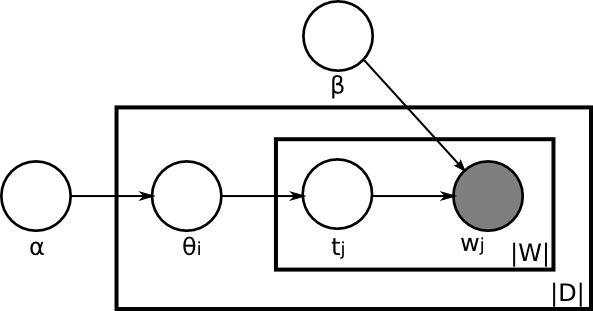
\includegraphics[width=6.5cm, height=3.2cm]{Latent_Dirichlet_allocation.png}\\
%  \caption{Modelo gráfico LDA.} %\ref{joint:lda}.}
%  \label{fig:lda}
%\end{figure}


% Assim como o Naïve Bayes, o LDA assume que palavras podem ser amostradas de acordo com distribuições multinomiais específicas, como evidencia a Fórmula \ref{multinomial}. A diferença é que, no LDA, cada palavra é amostrada a partir de uma \textbf{mistura de tópicos}; no Naïve Bayes, elas são geradas a partir de um só tópico (classe) \cite{gibbs-lingpipe}.

%, algo relativamente subjetivo. %ser bastante levando  

%Os significados dos tópicos em um LDA requerem uma interpretação posterior ao processamento. Esta interpretação baseia-se nas relações semânticas/temáticas entre as palavras que se associaram mais frequentemente a cada um deles. 


%- ou seja, não são identificados antes ou durante o processamento -cujos significados requerem  só podem ser interpretados após o processamento do modelo, observando-se  

% que, após o processamento, sintetizam um significado associado ao


%atribuir um significado a cada um deles apenas observando as relações entre as palavras associadas com mais destaque. Para o LDA, os tópicos não são, portanto, pré-identificados antes do processamento, requerendo uma interpretação posterior e subjetiva de seus significados. %Neste sentido, o modelo é útil para identificar padrões contidos em documentos de texto.  




%O cálculo destas probabilidades também envolve integrais difíceis, ou mesmo impossíveis, de resolver analiticamente, o que implica no uso de técnicas de amostragem e aproximação. A amostragem de Gibbs, descrita superficialmente na seção \ref{subsection:bayes}, é uma alternativa para a geração de valores para variáveis aleatórias contidas no modelo \cite{gibbs-lingpipe}, sendo utilizada nos experimentos com LDA conduzidos neste projeto. 

%Quando um método de classificação é aplicado a um conjunto de documentos, a interpretação do resultado é imediata: cada documento estará associado a uma única classe. No caso do modelo de tópicos LDA, a interpretação do resultado é mais subjetiva. É preciso observar as palavras que se associam com maior probabilidade a cada tópico, buscando algum tipo de semelhança entre elas, para inferir seus significados. 


% o agrupamento de palavras como \emph{beef}, \emph{sauce} e \emph{cheese} em torno de um mesmo tópico indica o bom funcionamento do LDA%As palavras associadas a cada tópico siderando que as receitas pertencem à culinária tradicional dos Estados Unidos. O primeiro tópico pode ser interpretado como \textbf{Receitas com Carne}, pois associa ingredientes comumente consumidos  
%\textbf{Análise}

% do envolvendo uma ou mais palavras associadas a uma \emph{tag} particular. 
%O resultado de um método de classificação consiste em associar cada documento de um conjunto Diferentemente de métodos de classificação, cujo resultado pode ser interpretado de forma obj

%Assim como discutido na seção \ref{subsection:bayes}, 
% tópicos é fixada multinomial  \ensure\ensuremath{d} se associa a tópicos \ensuremath{t \in T} com probabilidades diferentes, o que é determinado pela escolha de uma distribuição de probabilidade sobre os tópicos. Em seguida, cada tópico é tratado como uma distribuição sobre palavras e cada palavra \ensuremath{w_i} de \ensuremath{d} se associa a eles de acordo com estas distribuições. A probabilidade da \ensuremath{i}-ésima palavra de \ensuremath{d} pode ser calculada como 

%P(wi) = sum P(wi | ti = j) P(ti = j), j de 1 a T. 

%onde ti é uma variável latente - ou seja, cujo valor não é observável, mas sim inferido - referente a um tópico, P(wi | ti = j) é a probabilidade de wi se associar ao tópico j e P(ti = j) é a probabilidade de se obter o tópico j na distribuição fixada para o documento \ensuremath{d} \cite{pnas}.

 %\textbf{Falar das receitas.}
%\textbf{Falar do uso de Gibbs Sampling para inferência}


%\subsection{L-LDA}



%Como o cenário de classificação envolve documentos de teste, cujas classes não são informadas ao classificador, uma saída para utilizar adequada deve-se inicialmente amostrar uma classe para cada % o cálculo desses valores se torna bastante complexo. É necessário, portanto, utilizar alguma técnica de amostragem para estimá-los. Para este projeto, o método escolhido foi o \textbf{Gibbs Sampling}, por ser simples de implementar e obter boas estimativas em um curto espaço de tempo. A técnica será apresentada brevemente nesta seção

%Não é possível obter os valores de \ensuremath{\phi} 
%A fim de se buscar estimativas para o conjunto de parâmetros que melhor se adaptem a \ensuremath{D}, Os valores de \ensuremath{\phi}, entretanto, não são usados diretamente na classificação. Em vez disso, %gera-se o documento baseando-se em seus hiperparâmetros e em informações extraídas do corpus, obtendo-se estimativas

%O gibbs sampling só é necessário quando você
%quer calcular os parâmetros P(tk|c) e P(c) usando, além dos documentos
%rotulados, documentos não rotulados. O fato de de repente o modelo
%virar um mixture model cria problemas de não-identificabilidade, e as
%somas e produtos que entram nas integrais complicam as coisas
%bastante.

%Esses valores podem ser estimados para documentos de \ensuremath{D''} de acordo com algum método de amostragem. Para esse projeto, o método escolhido foi o \textbf{Gibbs Sampling}, pe


%as equações \ref{classe2} e \ref{palavra} \cite{gibbs-lingpipe}. Antes de tudo, entretanto,  Por questões de escopo, suas derivações não serão apresentadas nessa monografia. 



%\begin{equation}
%\label{palavra}
%\ensuremath{P(w_t | c_j ; \theta') \eq \frac{1 + \sum_{i = 1}^{|D'|}z_{ij}N(w_t, d_i)}{\sum_{s = 1}^{|V|}\sum_{i = 1}^{|D'|}z_{ij}N(w_s, d_i)}}
%\end{equation}

%onde \ensuremath{z_{ij}} é dado pela classe \ensuremath{y_i} de \ensuremath{d_i}: 1 quando \ensuremath{y_i = c_j} e 0 em caso contrário. \ensuremath{N(w_t, d_i) é o número de vezes que a palavra \ensuremath{w_t} ocorre em \ensuremath{d_i}. A esse valor, dá-se o nome de \textbf{contagem} da palavra \ensuremath{w_i} em \ensuremath{d_i}, informação muito utilizada nos métodos de classificação de documentos por perspectiva. O Capítulo \ref{chap3}, inclusive, é totalmente dedicado à discussão do uso dessa informação para essa tarefa. A probabilidade de se obter uma classe \ensuremath{c_j}, por sua vez, é dada por%where N(wt , di ) is the count of the number of times word wt occurs in document di
%and where zij is given by the class label: 1 when yi = cj and otherwise 0.



%Para a classificação de documentos ser bem-sucedida, os valores de \ensuremath{\phi} devem modelar \ensuremath{D} da melhor forma possível. Isso significa que não basta amostrá-los de acordo com os hiperparâmetros \ensuremath{\{\alpha, \beta, \gamma_1, ..., \gamma_|D|\}} para obter boas estimativas para os dois termos no numerador de \ref{teorema-bayes}. É preciso estimá-los de acordo com informações extraídas dos próprios documentos. % dessa equação. e  Além disso, assume-se, no modelo Naïve Bayes, que as palavras dos documentos são condicionalmente independentes, de modo que a equação \ref{teorema-bayes} pode ser reescrita como

%O modelo Naïve Bayes é composto de um conjunto de parâmetros \ensuremath{\theta}, conforme discutido na seção \ref{subsection:naive}. Para identificar a classe \ensuremath{y_i} de um documento \ensuremath{d_i \in D''}, é preciso estimar inicialmente valores para esses parâmetros, gerando um novo conjunto \ensuremath{\theta'}. Embora seja possível considerar apenas o conjunto de treinamento 



%Essas estimativas devem maximizar \ensuremath{P(\theta | D')} ou \ensuremath{P(\theta | D)}. Pelo Teorema de Bayes, tem-se que, no primeiro caso, \ensuremath{P(\theta | D') \prop P(D' | \theta)P(\theta)}. Para se maximizar essa relação, deve-se resolver um sistema de derivadas parciais do \ensuremath{log(P(\theta | D')} utilizando-se uma técnica denominada Maximum a Posteriori (MAP) \cite{nigam}, tópico que não será abordado nessa monografia. É suficiente saber que essa maximização conduz às expressões \ref{palavra} e \ref{classe2}, muito importantes para a compreensão dos próximos capítulos\footnote{Essas expressões podem variar um pouco, a depender do método utilizado para derivá-las. As versões apresentadas aqui foram retiradas da dissertação de Kamal Nigam \cite{nigam}.}. A probabilidade de se obter uma palavra \ensuremath{w_t \in V}, fixada uma classe \ensuremath{c_j}, é dada por



%O segundo caso é análogo.}



%O processo de maximização, em ambos os casos, é relativamente complexo, fugindo ao escopo dessa monografia. Ele conduz, entretanto, a expressões bastante simples matematicamente, utilizadas na implementação dos classificadores%obtidas, entretanto, são bastante simples matematicamente % Basicamente, elas são razões entre % baseiam exclusivamente no número de vezes que cada palavra ocorre em um documento ou em uma classe %relacionam o número de ocorrências de cada palavra ocorre em um documento ou em uma classe% utilizadas efetivamente pelos classificadorsentretanto, são  %O primeiro caso é mais simples, pois envolve apenas documentos para os quais já se conhecem as classes. % Por este motivo, ele será discutido inicialmente.% O segundo caso requer mais informações, sendo discutido % \ensuremath{\theta'}% que maximizem \ensuremath{arg max_j P(y_i = c_j | d_i ; \theta')}. Aplicando-se o Teorema de Bayes, tem-se que
 
                                                 %This is the value of θ that is most probable given the evidence of the training data and a prior.


%\begin{equation}
%\label{palavra}
%\ensuremath{P(w_t | c_j ; \theta') \eq \frac{1 + \sum_{i = 1}^{|D'|}z_{ij}N(w_t, d_i)}{\sum_{s = 1}^{|V|}\sum_{i = 1}^{|D'|}z_{ij}N(w_s, d_i)}}
%\end{equation}

%onde \ensuremath{z_{ij}} é dado pela classe \ensuremath{y_i} de \ensuremath{d_i}: 1 quando \ensuremath{y_i = c_j} e 0 em caso contrário. \ensuremath{N(w_t, d_i) é o número de vezes que a palavra \ensuremath{w_t} ocorre em \ensuremath{d_i}. A esse valor, dá-se o nome de \textbf{contagem} da palavra \ensuremath{w_i} em \ensuremath{d_i}, informação muito utilizada nos métodos de classificação de documentos por perspectiva. O Capítulo \ref{chap3}, inclusive, é totalmente dedicado à discussão do uso dessa informação para essa tarefa. A probabilidade de se obter uma classe \ensuremath{c_j}, por sua vez, é dada por%where N(wt , di ) is the count of the number of times word wt occurs in document di
%and where zij is given by the class label: 1 when yi = cj and otherwise 0.

%\begin{equation}
%\label{classe2}
%\ensuremath{P(c_j | \theta') \eq \frac{1 + \sum_{i = 1}^{|D'|}z_{ij}}{|C| + |D'|}}
%\end{equation}

%Não é possível aplicar as equações \ref{palavra} e \ref{classe2} diretamente no segundo caso, pois o classificador não sabe que classes correspondem aos documentos de \ensuremath{D''}. Para se obter boas estimativas para \ensuremath{\theta} nesse caso, uma saída é utilizar um método de amostragem, como \ensuremath{Gibbs Sampling}. %- e, consequentemen neste caso, conduzindo  % \ensuremath{\theta'} considerando todos os documentos de \ensuremath{D}, uma saída é utilizar um método de amostragem, como Gibbs Sampling. amostrar, inicialmente, a classe de cada \ensuremath{d \in D''}, considerando as distribuições de probabilidade \ref{theta_c} e \ref{classe} apresentadas na seção \ref{subsection:naive}. Neste momento, é interessante que a escolha de qualquer classe seja equiprovável, dado que não se sabe quantos documentos de \ensuremath{D''} efetivamente pertencem a cada uma delas. Com todos os documentos rotulados, é possível obter uma estimativa para \ensuremath{P(\theta | D)}, mas nada garante que ela seja a melhor possível. O que deve ser feito, neste caso, é reclassificar os documentos de \ensuremath{D''} diversas vezes, até que se estabilizem os valores estimados para \ensuremath{\theta} - ou seja, até que o modelo convirja. Esses valores configuram uma estimativa ótima para \ensuremath{\theta}. Para reclassificar os documentos de \ensuremath{D''}

%utilizar as equações \ref{palavra} e \ref{classe2}, trocando \ensuremath{D'} por \ensuremath{D}. O que se obtêm, entretanto, não são estimativas ideais para \ensuremath{w_t} e \ensuremath{c_j}, pois os parâ


%Entretanto, essa primeira classificação não é suficiente, pois os parâmetros obtidos não necessariamente maximizam \ensuremath{P(\theta | D)}. Para se obter os melhores parâmetros que modelam \ensuremath{D} % e utilizar esses valores para 


%Dizer que isso é preferível pois modela melhor.

 %  parte dos documentos contidos em \ensuremath{D} (\ensuremath{D''}). %o segundo caso, antes de resolver a maximização que conduz a equações análogas a \ref{palavra} e \ref{classe}, é preciso estimar valores iniciais  % tamb
%the highest posterior probability, arg maxj P(yi = cj |di ; θ)


% O objetivo inicial do classificador Naïve Bayes, portanto, é obter um \ensuremath{\theta} que maximize \ensuremath{P(\theta | D')} ou \ensuremath{P(\theta | D)}. No primeiro caso, tem-se, utilizando o Teorema de Bayes, que

%\begin{equation}
%\label{gerando-theta}
%\ensuremath{P(\theta | D') \eq \frac{P(D'|\theta)P(\theta)}{P(D')} 
%\end{equation}

%A maximização dessa equação é bastante complexa, fugindo completamente do escopo dessa monografia. A expressão obtida, entretanto, é fundamental para a compreensão dos próximos capítulos


 %conjunto de valores para eles que 




%dor de documentos a partir dele. Esta seção trata de documentos de texto em particular, por se tratarem do objeto básico de estudo deste projeto. 
%Sabe-se que, em um Naïve Bayes, assume-se que as as características em um documento são condicionalmente independentes, o que equivale a afirmar, por exemplo, que a presença de uma palavra em um documento de texto não é informativa sobre a presença de nenhuma outra. Apesar desta hipótese simplificar bastante a estrutura linguística de um texto, classificadores construídos a partir do modelo Naïve Bayes, denominados classificadores Naïve Bayes, reportam um bom desempenho em várias tarefas de classificação baseadas em palavras \cite{naive-at-forty} \cite{mccallum-naive}.

%Dados um documento \ensuremath{d} pertencente a um conjunto de documentos \ensuremath{D}, todas as palavras distintas de \ensuremath{D}, \ensuremath{F_1, ..., F_k}, uma variável aleatória \ensuremath{c}, que representa as possíveis classes de \ensuremath{d}, e um vetor \ensuremath{v_d}, em que cada posição corresponde a uma de suas \ensuremath{n} palavras, tem-se que
 

%conforme discutido anteriormente na seção \ref{subsection:naive}. Um classificador Naïve Bayes deve rotular o documento \ensuremath{d} com o valor de \ensuremath{c} que maximiza a equação \ref{eq2:bayes}. Como o denominador na equação \ref{eq2:bayes} é o mesmo para todas as classes, ele pode ser ignorado nestes cálculos.

%Normalmente, classificadores Naïve Bayes são utilizados de forma semi-supervisionada. Isto significa que eles são submetidos a uma etapa de treinamento, na qual aprendem as classes associadas a alguns documentos, e a uma etapa de classificação, na qual devem simular o processo gerador destes documentos e utilizar esta informação para classificar outros. Basicamente, as informações aprendidas na etapa de treinamento modelam as distribuições das palavras de \ensuremath{D} por classe, gerando parâmetros para as distribuições de probabilidade envolvidas na classificação de outros documentos. 


%O número de iterações para amostragem de tópicos e palavras, em todos os experimentos, foi fixado em 100.

% a amostragem da equação \ref{eq:bayes} foi fixado em 500.

% classificando outros                        Dado que tenho exemplos de texto de cada classe. O
%que posso inferir sobre o processo gerador destes textos


%                              e                  o classificador reporta
%o melhor desempenho em v ́rias tarefas de classifica ̧ ̃o. Este fenˆmeno  ́
%                        a                         ca

 
%\begin{algorithm}
%\ensuremath{z^{(0)}} \gets \ensuremath{\langle z_1^{(0)}, \ldots, z_k^{(0)}\rangle}
%\FOR{\ensuremath{t = 1} to \ensuremath{T} do}
 % \FOR{\ensuremath{i = 1} to \ensuremath{k} do}
 %   \ensuremath{z_i^{(t + 1)} ~ P(Z_i | z_1^{(t + 1)}, \ldots, z_{i - 1}^{(t + 1)}, z_{i + 1}^{(t)}, \ldots, z_k^{(t)})}
 % \ENDFOR
%\ENDFOR

%\end{algorithm}


%Além disso, você deveria começar a descrever o naive bayes falando que
%ele é um modelo generativo e que assume independência condicional das
%features dado as classes. Dizer que naive bayes aproxima P(vetor(d),c)
%como sendo P(c) Produtorio(P(di|c), o que é a mesma coisa que dizer
%que as palavras são condicionalmente independentes dado as classes,
%mostrar como vc faz pra usar isso pra classificar, usando P(c|d)  =
%P(c,d)/P(d), e que como P(d) independe da classe pode ser ignorado se
%você quer encontrar a melhor classe. Daí você deveria especificar de
%onde vêm essas probabilidades, colocando uma prior Beta(alpha, alpha)
%em P(c) e uma prior Dirichlet(alpha) em P(tk|c).

%Dado um conjunto de documentos \ensuremath{D} e um conjunto de classes \ensuremath{C}, o classificador Naïve Bayes estima, através da aplicação do Teorema de Bayes,  a probabilidade de cada \ensuremath{d \in D} ser de cada uma das classes \ensuremath{c \in C}. Com estas probabilidades calculadas, o classificador determina, para todo \ensuremath{d}, qual é a classe \emph{c} a que ele estará associado. Esta classe pode, por exemplo, ser aquela para a qual a probabilidade obtida foi simplesmente a mais alta \cite{durant-smith} \cite{naive-forty}.

%Este tipo de classificador parte da ideia de que as informações presentes em um documento, utilizadas na determinação de sua classe, são independentes entre si. No caso de um documento de texto, assume-se que a presença ou ausência de um termo - uma palavra ou uma sequência de palavras - é independente da presença ou ausência de qualquer outro. Definida esta hipótese, a probabilidade de que um documento \emph{d} seja de uma classe \emph{c} é tal que

%\begin{equation}
%\label{eq1}
%\ensuremath{P(c|d) \propto P(c)\prod_{k=1}^{t_d}P(t_k|c)}  
%\end{equation} 

%onde \ensuremath{P(t_k|c)} é a probabilidade condicional do termo \ensuremath{t_k}  ocorrer em um documento da classe \ensuremath{c},  \ensuremath{P(c)} é a probabilidade a priori de um documento qualquer pertencer à classe \ensuremath{c} e \ensuremath{t_d} é o número de termos em \emph{d} \cite{stanford-IRbook}.

%As probabilidades envolvidas na relação \ref{eq1} contêm integrais díficeis ou mesmo impossíveis de se calcular analiticamente. Para calcular \ensuremath{P(c|d)}, portanto, utiliza-se aproximações obtidas através de técnicas de amostragem. Uma destas técnicas, comum na literatura de Aprendizado de Máquina e empregada neste projeto, é a amostragem de Gibbs. Em uma iteração da amostragem, a técnica condiciona as probabilidades calculadas para um documento \ensuremath{k} às classificações obtidas para os \ensuremath{k - 1} documentos anteriores \cite{resnik-gibbs}. A técnica está descrita, de forma básica, no algoritmo \textbf{X (o algorithm2e.sty tá dando pau)}.
                             % The basic idea in Gibbs sampling is that, rather than probabilistically picking
%the next state all at once, you make a separate probabilistic choice for each of the k dimensions, where each
%choice depends on the other k − 1 dimensions.


%A hipótese de independência entre os termos, razão pela qual o Naïve Bayes tem este nome\footnote{Naïve é uma palavra de origem francesa que significa "ingênua"}, simplifica bastante a estrutura da informação contida nos documentos. Ainda assim, o classificador costuma apresentar boas performances em categorização de textos, sendo utilizado, por exemplo, como base metodológica para alguns filtros de \emph{spam} \cite{paul}. Para melhorar o desempenho do Naïve Bayes, é comum fixar um conjunto de documentos previamente classificados de forma correta e utilizar a informação sobre suas classes na determinação das classes de outros documentos. Ao conjunto de documentos previamente classificados, dá-se o nome de \textbf{conjunto de treinamento}; ao conjunto de documentos a serem classificados, \textbf{conjunto de teste}.

 %Através do uso de Amostragem de Gibbs, a cada iteração se obtém uma aproximação melhor O número de amostras coletadas envolvendo cada classe foi fixado em 500. 
 
 
%     We shall assume for the moment that the training data set is linearly separable in
%feature space, so that by definition there exists at least one choice of the parameters
%w and b such that a function of the form (7.1) satisfies y(xn ) > 0 for points having
%tn = +1 and y(xn ) < 0 for points having tn = −1, so that tn y(xn ) > 0 for all
%training data points.


%Suppose some given data points each belong to one of two classes, and the goal is to decide which class a new data point will be in. In the case of support vector machines, a data point is viewed as a p-dimensional vector (a list of p numbers), and we want to know whether we can separate such points with a p − 1-dimensional hyperplane. This is called a linear classifier. There are many hyperplanes that might classify the data. One reasonable choice as the best hyperplane is the one that represents the largest separation, or margin, between the two classes. So we choose the hyperplane so that the distance from it to the nearest data point on each side is maximized. If such a hyperplane exists, it is known as the maximum-margin hyperplane and the linear classifier it defines is known as a maximum margin classifier.

% cada documento do corpus é representado como um vetor \ensuremath{x} em um espaço euclidiano \ensuremath{\mathbb{R}^M}. Na etapa de treinamento, \ensuremath{N} documentos, com suas respectivas classes \ensuremath{c_0} ou \ensuremath{c_1}, são apresentadas ao classificador, que deve aprender uma função e a classificação envolve o aprendizado de uma função que corte este hiperplano, dividindo os pontos em duas classes distintas. 




